\documentclass[10pt,hyperref={pdfpagelabels=true}]{beamer}

\mode<presentation>
{
  \usetheme[footline]{PISMshade}
  \setbeamercovered{transparent}
}

\usepackage{verbatim,amsmath,empheq,times,bm}
\usepackage[english]{babel}
\usepackage[utf8]{inputenc}

\usepackage{tikz}
\usepackage{hyperref}

\definecolor{dark red}{HTML}{E41A1C}
\definecolor{dark green}{HTML}{4DAF4A}
\definecolor{dark violet}{HTML}{984EA3}
\definecolor{dark blue}{HTML}{084594}
\definecolor{dark orange}{HTML}{FF7F00}
\definecolor{light blue}{HTML}{377EB8}
\definecolor{light red}{HTML}{FB9A99}
\definecolor{light violet}{HTML}{CAB2D6}

\setbeamercolor{boxed}{fg=black,bg=uaf yellow}

\newcommand{\CC}{\mathbb{C}}
\newcommand{\NN}{\mathbb{N}}
\newcommand{\RR}{\mathbb{R}}
\newcommand{\ZZ}{\mathbb{Z}}
\newcommand{\Acal}{\mathcal{A}}
\newcommand{\Bcal}{\mathcal{B}}
\newcommand{\Ccal}{\mathcal{C}}
\newcommand{\Ncal}{\mathcal{N}}
\newcommand{\Kcal}{\mathcal{K}}

\newcommand{\bF}{\mathbf{F}}
\newcommand{\bQ}{\mathbf{Q}}
\newcommand{\bU}{\mathbf{U}}

\newcommand{\bbU}{\bar{\bU}}

\newcommand{\bb}{\mathbf{b}}
\newcommand{\bu}{\mathbf{u}}
\newcommand{\bv}{\mathbf{v}}
\newcommand{\bx}{\mathbf{x}}

\newcommand{\Div}{\nabla\cdot}
\newcommand{\eps}{\epsilon}
\newcommand{\grad}{\nabla}
\newcommand{\lap}{\triangle}
\DeclareMathOperator{\trace}{tr}
\renewcommand{\bar}{\overline}

\newcommand{\ddx}[1]{\frac{\partial #1}{\partial x}}
\newcommand{\ddy}[1]{\frac{\partial #1}{\partial y}}
\newcommand{\pp}[2]{\frac{\partial #1}{\partial #2}}
\newcommand{\ppt}[1]{\frac{\partial #1}{\partial t}}
\newcommand{\ppT}[1]{\frac{\partial #1}{\partial T}}
\newcommand{\ppx}[1]{\frac{\partial #1}{\partial x}}
\newcommand{\ppy}[1]{\frac{\partial #1}{\partial y}}
\newcommand{\ppz}[1]{\frac{\partial #1}{\partial z}}
\newcommand{\ppxx}[1]{\frac{\partial^2 #1}{\partial x^2}}
\newcommand{\ppzz}[1]{\frac{\partial^2 #1}{\partial z^2}}

\newcommand{\Tnorm}[1]{\left|\!\left|\!\left|#1\right|\!\right|\!\right|}
\newcommand{\rhow}{\rho_{\text{w}}}
\newcommand{\Wq}{W^{1,q}(\Omega)}
\newcommand{\half}{\frac12}

%\setbeamercolor{redtext}{fg=red!80!black}
\setbeamercolor{redtext}{fg=red!94!black}
%\setbeamercolor{greentext}{fg=green!80!black}
\setbeamercolor{greentext}{fg=green!60!black}
%\setbeamercolor{bluetext}{fg=blue!70!black}
\setbeamercolor{bluetext}{fg=blue!90!black}
\setbeamercolor{yellowtext}{fg=yellow!95!black}
\setbeamercolor{orangetext}{fg=yellow!50!red}

\newcommand{\green}{\usebeamercolor[fg]{greentext}}
\newcommand{\blue}{\usebeamercolor[fg]{bluetext}}
\newcommand{\red}{\usebeamercolor[fg]{redtext}}

\renewcommand{\L}{\emph{Left}}
\newcommand{\R}{\emph{Right}}


\newcommand{\contactslipslide}[1]{
\begin{frame}{#1 sheets vs.~streams vs.~shelves}

\begin{columns}
\begin{column}{0.35\textwidth}
\small
\begin{itemize}
\small
\item non-sliding portions of ice sheets flow by shear deformation
\item ice streams slide: \alert{contact slip}
\item ``ice shelves'' are floating thick ice
  \begin{itemize}
  \scriptsize
  \item[$\circ$] also \alert{contact slip}
  \end{itemize}
\end{itemize}
\end{column}

\begin{column}{0.65\textwidth}

\hfill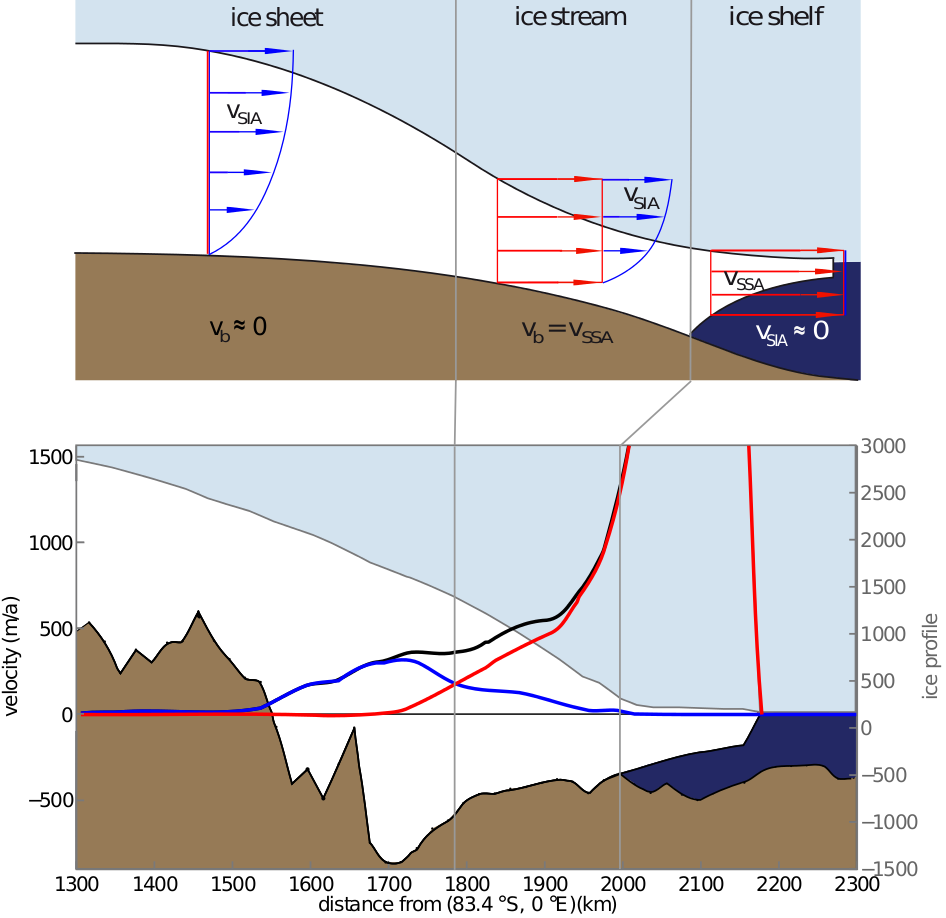
\includegraphics[width=0.95\textwidth]{siassacartoon-lambert}

\begin{center}
\vspace{-0.18in}
\tiny [Lambert glacier and Amery ice shelf, Antarctic]
\end{center}
\end{column}
\end{columns}
\end{frame}
}



\title{Modeling flowing ice sheets \\ \dots as applied math}

\author[Bueler]{Ed Bueler}

\institute[UAF]{
  \tiny Dept of Mathematics and Statistics \\

  University of Alaska Fairbanks
}

\date{\tiny 18 May, 2018}


\setbeamerfont{date}{size=\scriptsize}

\subject{ice sheets, glaciers, numerical analysis, applied mathematics}


\AtBeginSection[]
{
  \begin{frame}<beamer>
    \frametitle{Outline}
    \tableofcontents[currentsection,hideallsubsections]
  \end{frame}
}


\begin{document}
\graphicspath{{../../old/commonfigs/}{../../figures/}}

\begin{frame}
  \titlepage
  \begin{center}
  \tiny supported by NASA grants NNX13AM16G, NNX16AQ40G, NNX17AG65G 
  \end{center}
\end{frame}



% NO OUTLINE BECAUSE ONE APPEARS AT START OF EACH SECTION ?
%\begin{frame}
  %\frametitle{Outline}
  %\tableofcontents[hideallsubsections]
  % You might wish to add the option [pausesections]
%\end{frame}


\section[the alien view]{the alien physicist view of Greenland}

\setbeamertemplate{background canvas}{
     \tikz{\node[inner sep=0pt,opacity=1] {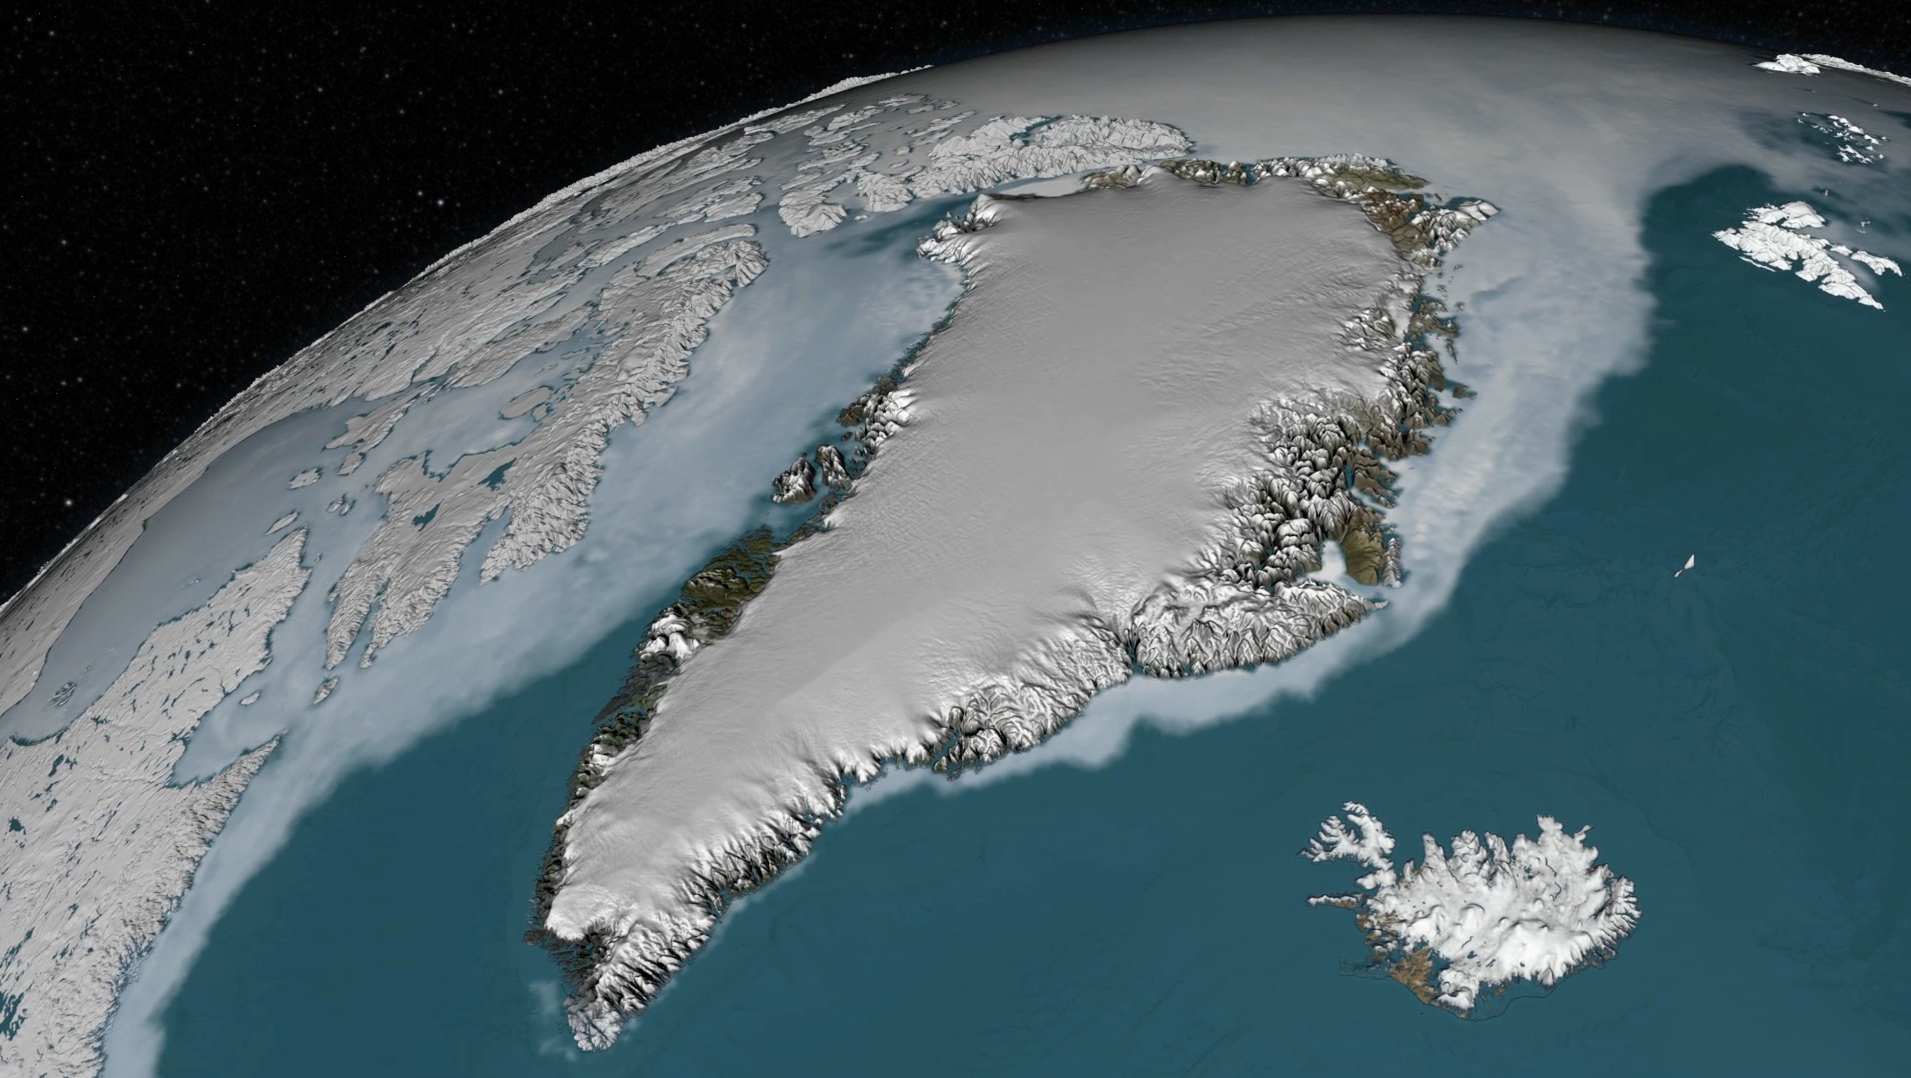
\includegraphics[height=\paperheight,width=\paperwidth]{nasa-mapping-greenland-ice-sheet}};}
} 

\begin{frame}{}

\only<2>{
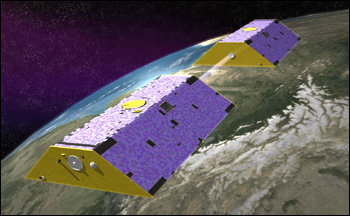
\includegraphics[width=0.3\textwidth]{grace-satellites}

\vfill \hfill 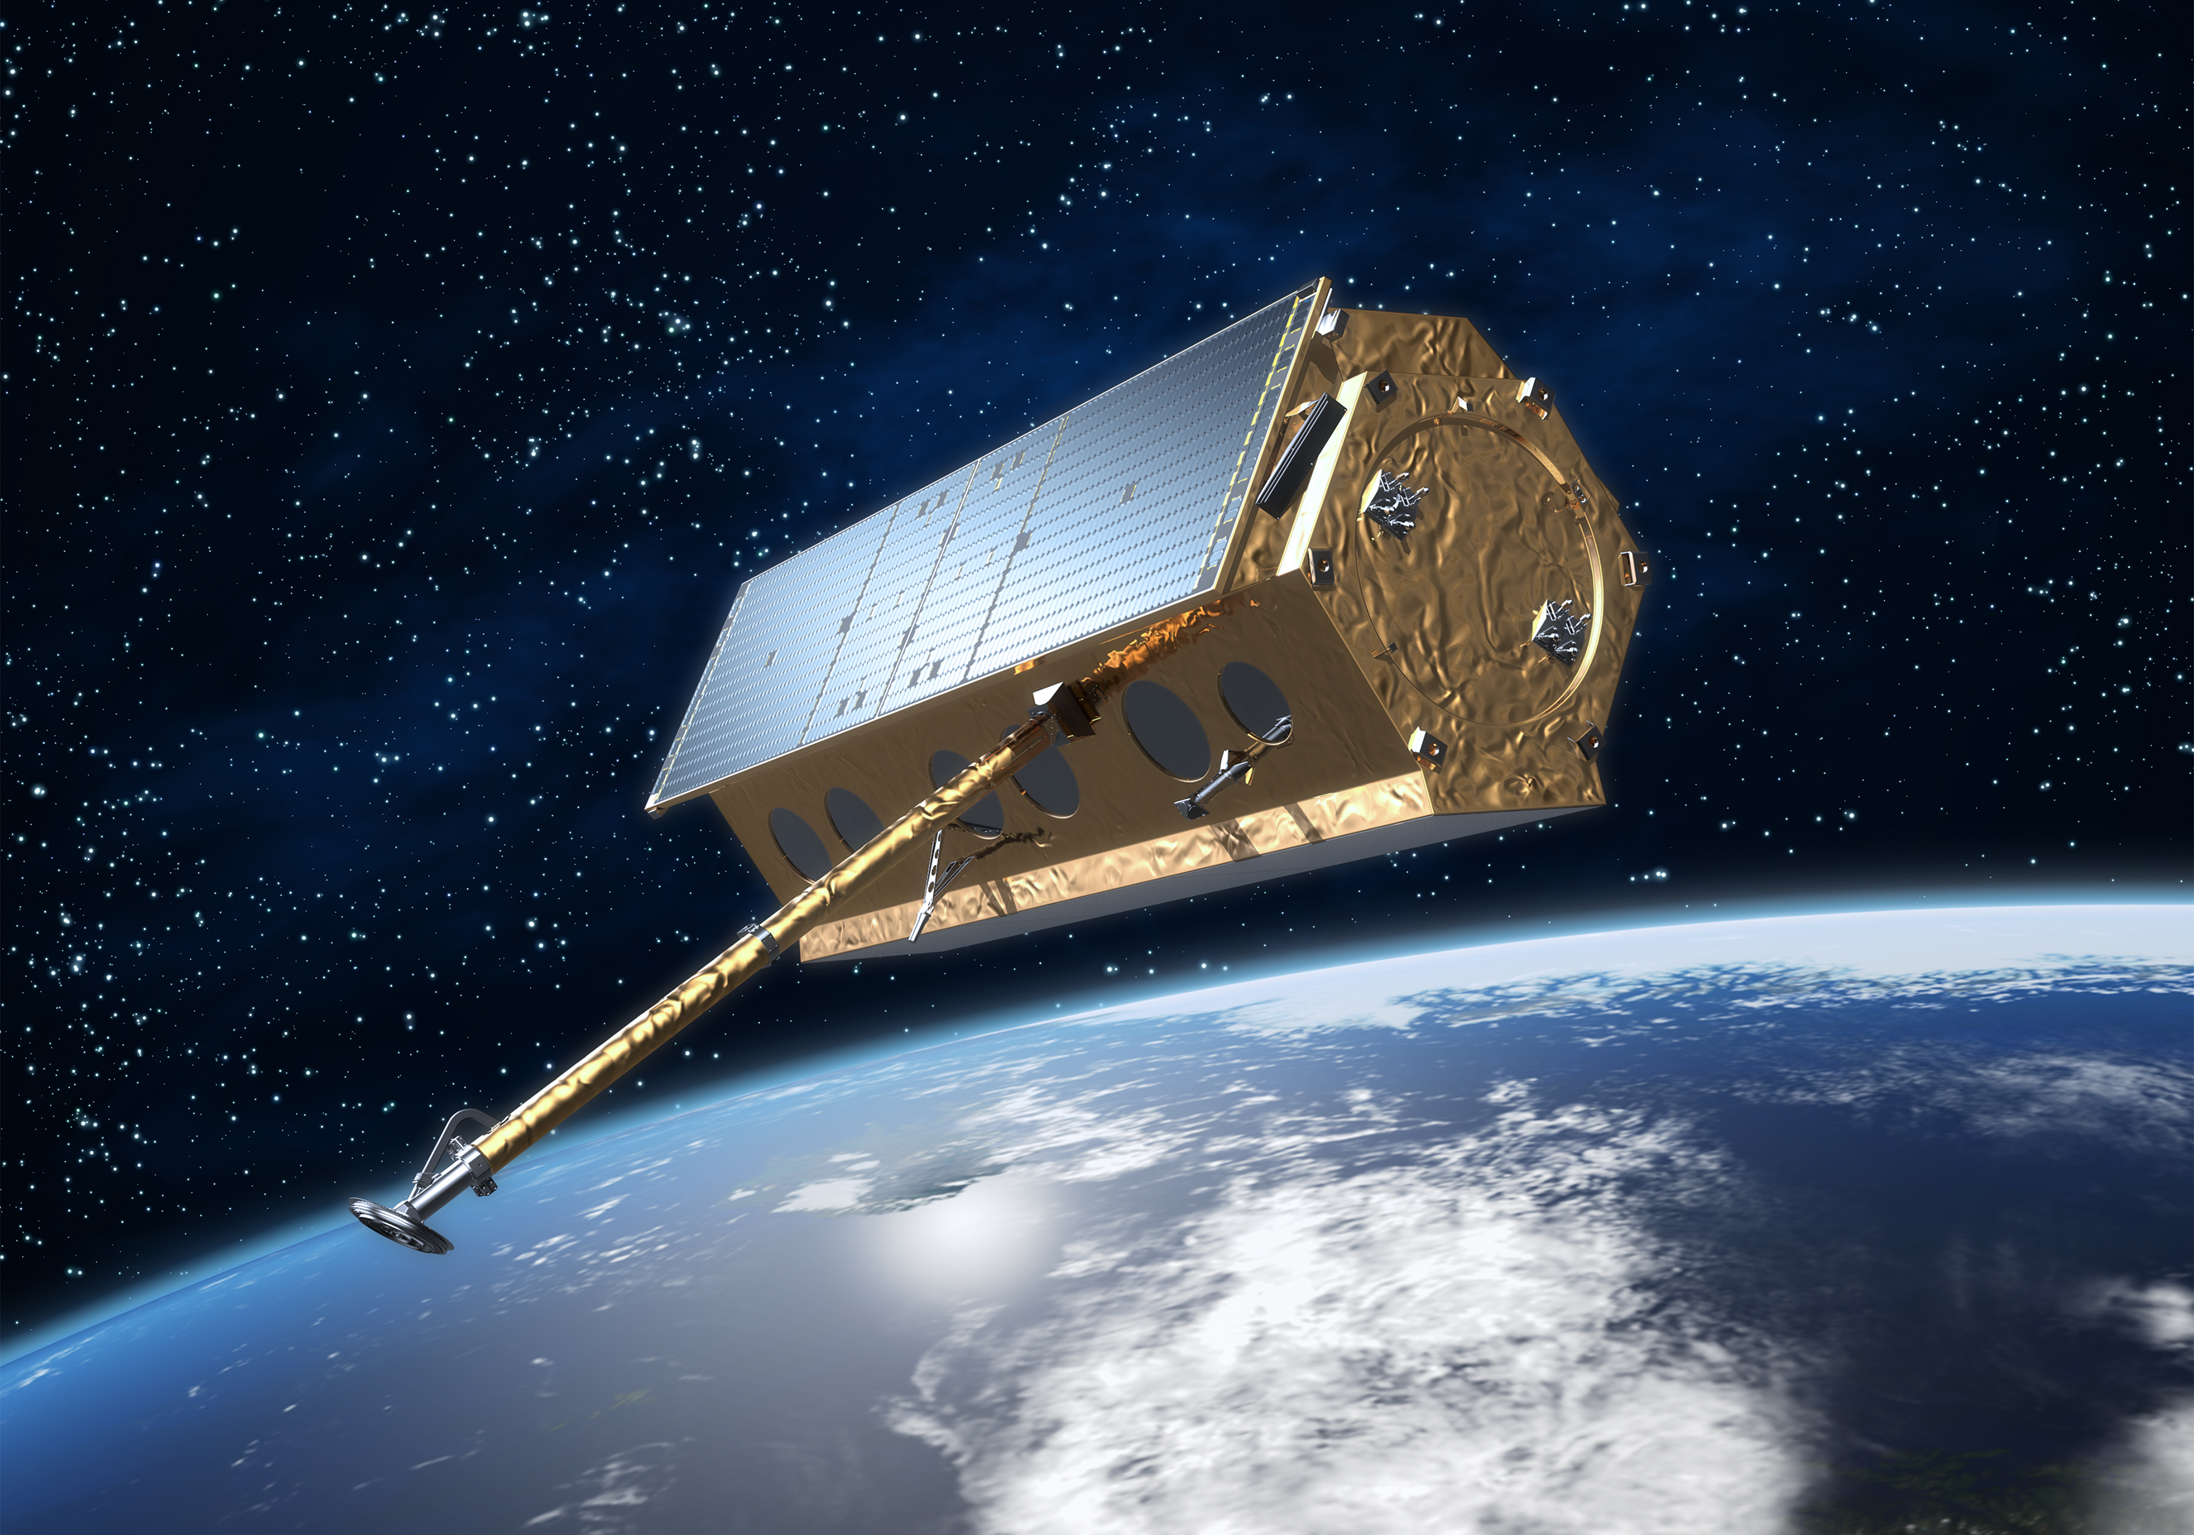
\includegraphics[width=0.3\textwidth]{TerraSAR_n}
}
\end{frame}


\setbeamertemplate{background canvas}{}

\begin{frame}{from space \dots}

\begin{columns}
\begin{column}{0.55\textwidth}
\begin{itemize}
\item one can measure gravity changes \phantom{foo bar}
\hfill \only<1>{\alert{show GRACE movie}}
\item<2-> one can measure surface movement (through \emph{synthetic aperture radar}) \phantom{foo bar baz} \hfill \only<2>{\alert{\dots at right}}
\item<3-> one can observe changes in ice extent \hfill \only<3>{\alert{\dots at right}}

\bigskip
\item<4> as a newly-arrived physicist observing Greenland, you would observe in the last decades:
    \begin{itemize}
    \item[$\circ$] the ice sheet has been losing mass
    \item[$\circ$] the flow pattern and ice extent around the outlet glaciers has changed
    \end{itemize}

\bigskip
\item<4> \dots whether or not you care about the causes
\end{itemize}
\end{column}
\begin{column}{0.45\textwidth}

\hfill \includegraphics<2>[width=0.78\textwidth]{greenland-overview-obsonly}
\hfill \includegraphics<3->[width=0.8\textwidth]{jib-front-1990-2005-change}
\end{column}
\end{columns}
\end{frame}


\section[intro to ice flow]{an introduction to flowing ice}


\begin{frame}{ice in glaciers is a viscous fluid}
\begin{columns}
\begin{column}{0.65\textwidth}
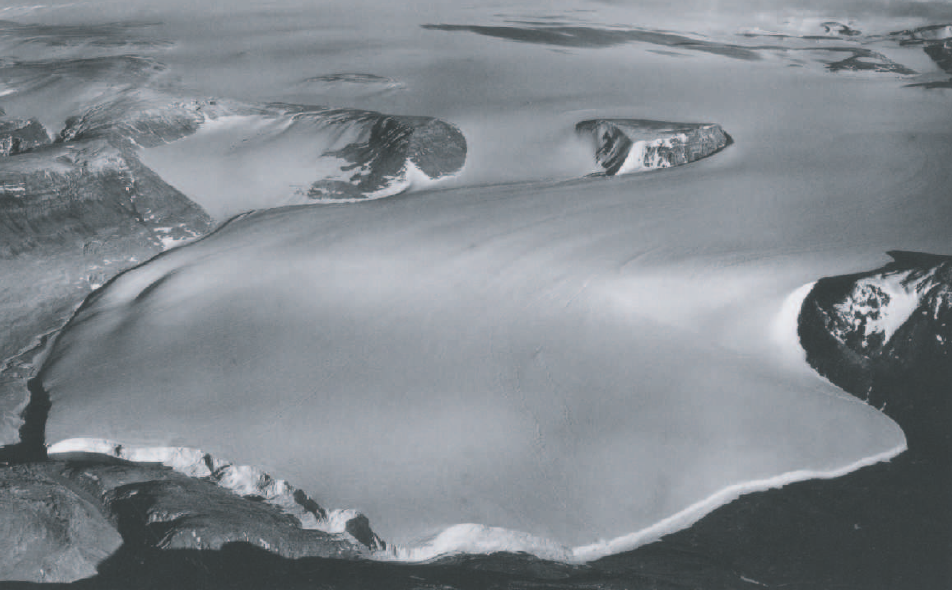
\includegraphics[width=1.0\textwidth]{polaris}
\end{column}
\begin{column}{0.35\textwidth}
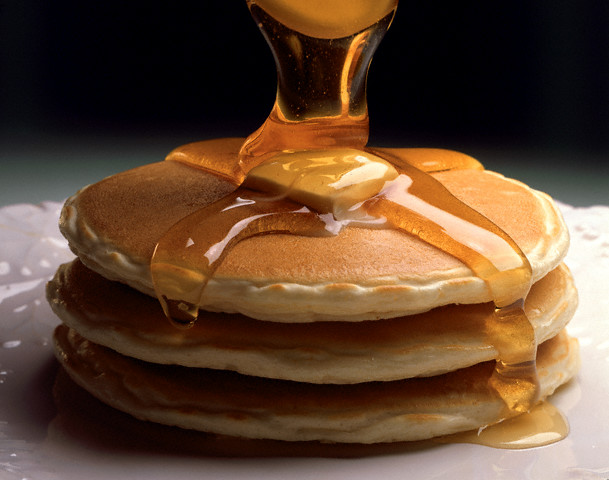
\includegraphics[width=1.0\textwidth]{pancakes}
\end{column}
\end{columns}

\bigskip
\begin{itemize}
\item glaciers and ice sheets are viscous flows at the large scale
  \begin{itemize}
  \item[$\circ$] at a smaller scale they are ice crystals
  \item[$\circ$] at yet-smaller scale they are molecules \dots atoms \dots quarks
  \end{itemize}
\item \emph{usage}: ``ice sheets'' are big, shallow glaciers
\end{itemize}
\end{frame}


\begin{frame}{ice sheets are shallow}

\begin{itemize}
\item cross section of Greenland ice sheet at $71^\circ$ N
  \begin{itemize}
  \item[$\circ$] {\color{dark green}{green}} and {\color{dark blue}{blue}}: vertically-exaggerated version
  \item[$\circ$] in {\color{dark red}{red}}: without vertical exaggeration
  \end{itemize}
\end{itemize}
\normalsize

  \begin{center}
    \tikz{\draw[<->] (0.0,-2.9) -- node [midway, left] {3500 m} (0.0,2.7);}  \quad 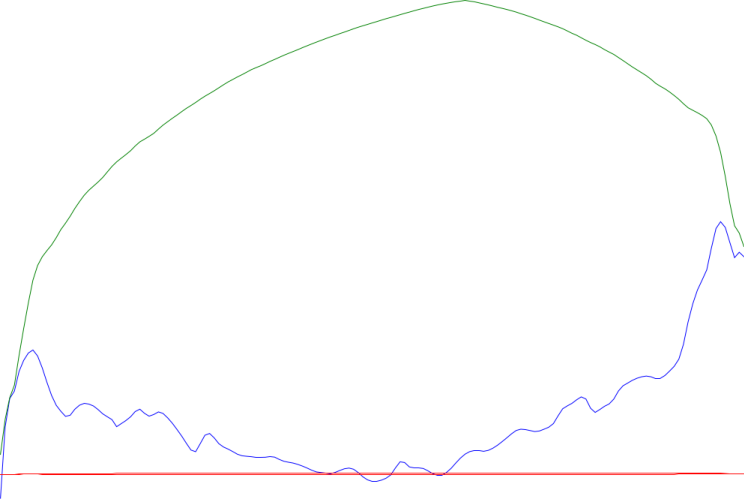
\includegraphics[width=0.7\textwidth]{greentransecttrimmed}
    
    \bigskip
    \qquad\qquad\qquad \tikz{\draw[<->] (-4.1,0.0) -- node [midway, below] {750 km} (4.1,0.0);}
  \end{center}
\end{frame}


\begin{frame}{what is a fluid?}

\begin{columns}
\begin{column}{0.6\textwidth}
\begin{itemize}
\item seriously, what is a fluid?
\item<2-> is it just a collection of particles?
\item<3-> a fluid is a mathematical abstraction
  \begin{itemize}
  \item<3->[$\circ$]   each smaller piece remains a fluid
  \item<3->[$\circ$]   a continuous function $y=f(x)$ is also such an abstraction
  \end{itemize}
\item<3-> a fluid is a \alert{model}
\item<4-> with primary variables:
  \begin{itemize}
  \item<4->[$\circ$]   velocity $\mathbf{u}(\bx,t)$
  \item<4->[$\circ$]   pressure $p(\bx,t)$
  \end{itemize}
\item<4-> gases, liquids, and \alert{ice} are all fluids (at big enough scale)
\end{itemize}
\end{column}
\begin{column}{0.4\textwidth}
\includegraphics<1>[width=\textwidth]{liquid}
\includegraphics<2>[width=\textwidth]{ivfluid}
\includegraphics<3>[width=\textwidth]{lighterfluidalpha}
\includegraphics<4>[width=\textwidth]{xinjiangglacier}
\end{column}
\end{columns}
\end{frame}


\begin{frame}{ice is a viscous fluid}

\begin{itemize}
\item these are fluids:
  \begin{itemize}
  \item[$\circ$] air
  \item[$\circ$] liquid water
  \item[$\circ$] syrup
  \item[$\circ$] glacier ice
  \end{itemize}
\item are usually modeled as \alert{incompressible viscous fluids}
\item a typical incompressible viscous fluid is described by Navier-Stokes equations:
\begin{align*}
\nabla \cdot \mathbf{u} &= 0 &&\qquad \text{\emph{incompressibility}} \\
\rho \left(\mathbf{u}_t + \mathbf{u}\cdot\nabla \mathbf{u}\right) &= -\nabla p + \nu \nabla^2 \mathbf{u} + \rho \mathbf{g} &&\qquad \text{\emph{stress balance}}
\end{align*}

\small
\item these equations are known to be hard
  \begin{itemize}
  \item[$\circ$] \$1 million Clay Institute prize for proving there are solutions in 3D \dots unclaimed for 18 years
  \item[$\circ$] but you've flown here on plane designed assuming we adequately understand them
  \end{itemize}
\end{itemize}
\end{frame}


\begin{frame}{ice is a weird viscous fluid}

\begin{itemize}
\item glacier ice is not a typical fluid!
\item for example, these are \alert{irrelevant in glacier flow}, but a big deal for weather and climate models of the atmosphere and ocean:
  \begin{itemize}
  \item[$\circ$] turbulence
  \item[$\circ$] convection
  \item[$\circ$] coriolis force
  \item[$\circ$] density variations
  \end{itemize}
\end{itemize}
\end{frame}


\begin{frame}{ice is a slow, shear-thinning fluid}

\begin{itemize}
\item recall Navier-Stokes:
\small
\begin{align*}
\nabla \cdot \mathbf{u} &= 0 &&\qquad \text{\emph{incompressibility}} \\
\rho \left(\mathbf{u}_t + \mathbf{u}\cdot\nabla \mathbf{u}\right) &= -\nabla p + \nu \nabla^2 \mathbf{u} + \rho \mathbf{g} &&\qquad \text{\emph{stress balance}}
\end{align*}
\normalsize
\item glacier ice fluid is
  \begin{enumerate}
  \item ``slow'' is a technical term:\footnote{the Froude number, the ratio of inertia to gravity, is approximately $10^{-15}$}

\vspace{-3mm}
    $$\rho \left(\mathbf{u}_t + \mathbf{u}\cdot\nabla \mathbf{u}\right) \approx 0 \qquad \iff \qquad \begin{pmatrix} \text{forces of inertia} \\ \text{are negligible} \end{pmatrix}$$
  \item non-Newtonian (shear-thinning):

    \begin{itemize}
    \item[$\circ$] viscosity $\nu$ is not constant
    \item[$\circ$] ``shear-thinning'' is a power law (Glen law):
        $$(\text{strain rate}) = A\, (\text{shear stress})^n$$
    \item[$\circ$] $1.8 < n < 4.0$ ?  \quad when in doubt: \alert{$n=3$}
    \end{itemize}
  \end{enumerate}
\end{itemize}
\end{frame}


\begin{frame}{equations for ice flow}

\begin{columns}
\begin{column}{0.65\textwidth}
\begin{itemize}
\item the \alert{standard model for ice flow} is Glen-Stokes:
\begin{align*}
\nabla \cdot \mathbf{u} &= 0 &&\text{\emph{incompressibility}} \\
0 &= - \nabla p + \nabla \cdot \tau_{ij} + \rho \mathbf{g} &&\text{\emph{stress balance}} \\
\mathbf{D}u_{ij} &= A \left|\tau_{ij}\right|^2 \tau_{ij} &&\text{\emph{Glen flow law}}
\end{align*}
\item notation:
  \begin{itemize}
  \item[$\circ$] $\tau_{ij}$ is deviatoric stress tensor
  \item[$\circ$] $\mathbf{D}u_{ij}$ is strain rate tensor
  \end{itemize}
\end{itemize}
\end{column}
\begin{column}{0.35\textwidth}

\hfill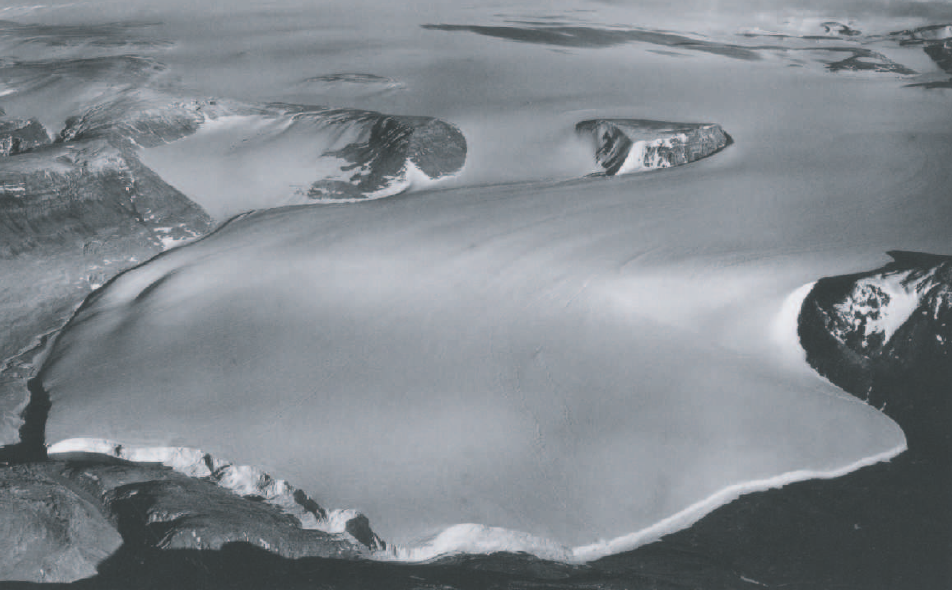
\includegraphics[width=0.9\textwidth]{polaris}

\bigskip\bigskip

\hfill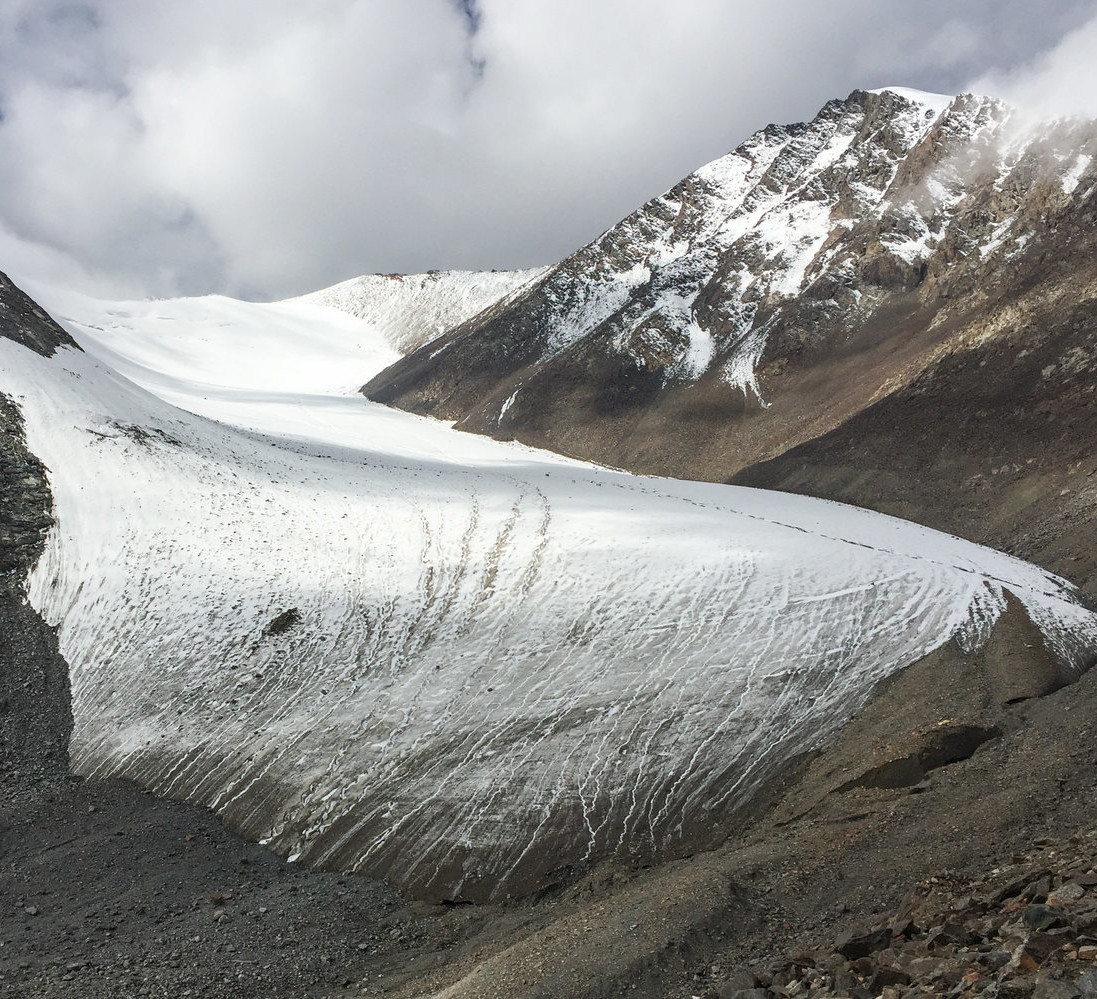
\includegraphics[width=0.9\textwidth]{xinjiangglacier}
\end{column}
\end{columns}
\end{frame}


\begin{frame}{wait \dots too many equations!}

\begin{itemize}
\item too many equations!
    \begin{itemize}
    \item[$\circ$] I know
    \end{itemize}
\item<2> what math is needed for numerical models of fluids like glaciers?
    \begin{itemize}
    \item[$\circ$] calc III
        \begin{itemize}
        \item partial derivatives, surface integrals, \dots
        \end{itemize}
    \item[$\circ$] linear algebra
        \begin{itemize}
        \item pretty much the fanciest trick you can program on a computer is to solve a linear system $A\bx = \bb$
        \end{itemize}
    \item[$\circ$] differential equations
        \begin{itemize}
        \item ODEs \emph{and} PDEs
        \end{itemize}
    \item[$\circ$] some computer programming
        \begin{itemize}
        \item Matlab or Python
        \item a course in numerical analysis is nice
        \end{itemize}
    \end{itemize}
\end{itemize}
\end{frame}


\section[big picture questions]{big picture questions for ice flow models}

\begin{frame}
  \frametitle{how much can sea level rise if ice sheets melt?}
  \framesubtitle{(big picture question 1)}

\begin{columns}
\begin{column}{0.6\textwidth}
\begin{itemize}
\item ice sheets are big masses of frozen water (mostly) sitting above the sea level
    \begin{itemize}
    \item[$\circ$] Greenland ice sheet mass is $2.9 \times 10^6$ Gt \quad $(\approx \text{km}^3)$ % = 2.93466 10^6 km^3  volume, from SeaRISE-Greenland 5km data
    \end{itemize}
\item if \emph{all} ice melts:
    \begin{itemize}
    \item[$\circ$] Antarctica: 61 m of sea level rise
    \item[$\circ$] Greenland: 7 m of sea level rise
    \item[$\circ$] all other glaciers: 35 cm of sea level rise
    \end{itemize}
\item so it would be good to know mechanisms of melt
\end{itemize}
\end{column}
\begin{column}{0.4\textwidth}

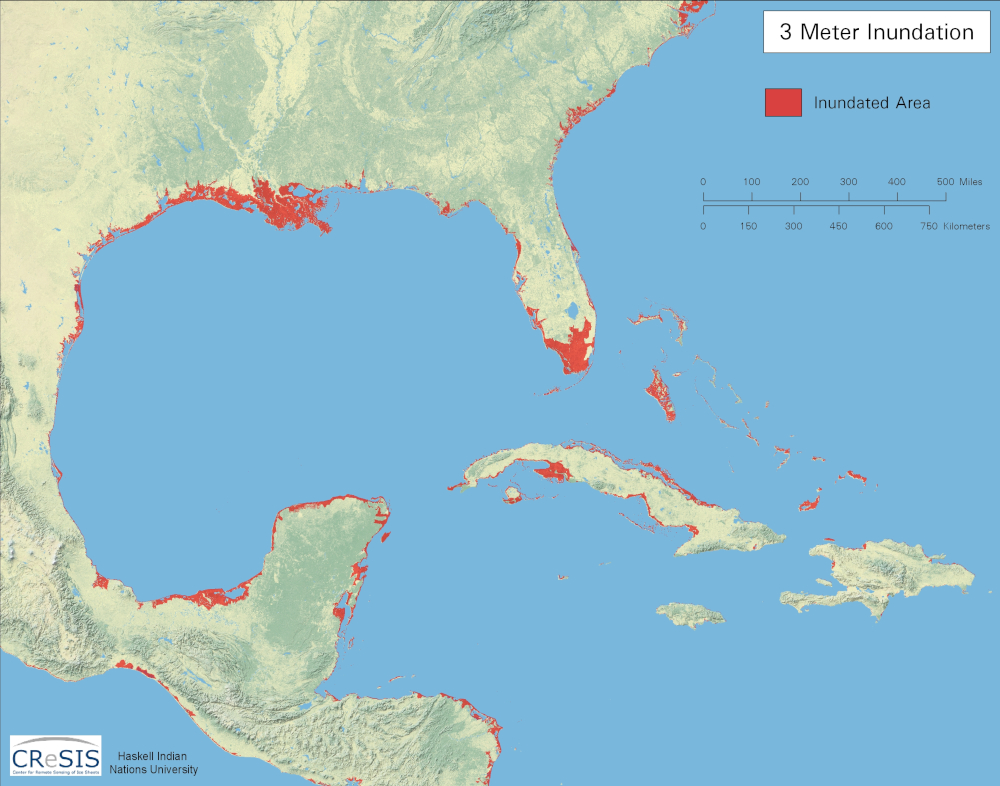
\includegraphics[width=0.95\textwidth]{southeastern_us_3m}
\end{column}
\end{columns}
\end{frame}


\begin{frame}
  \frametitle{how does flowing ice interact with climate?}
  \framesubtitle{(big picture question 2)}

\medskip
\small
\begin{itemize}
\item \emph{mass and energy inputs}: snow adds, sun heats, ocean heats
\item \emph{mass outputs}: surface melts, base melts, ice flows out (discharges)
\end{itemize}

\begin{center}
  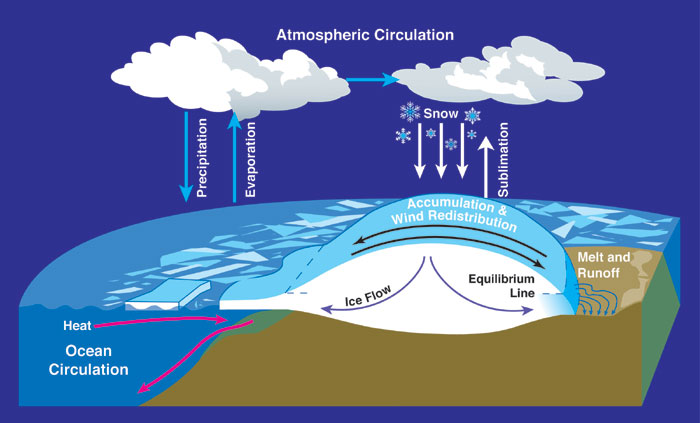
\includegraphics[width=0.75\textwidth]{mass-bal-atmos}
\end{center}
\end{frame}


\contactslipslide{}


\begin{frame}
  \frametitle{ice shelf versus sea ice}

\begin{center}
\vspace{-0.2in}

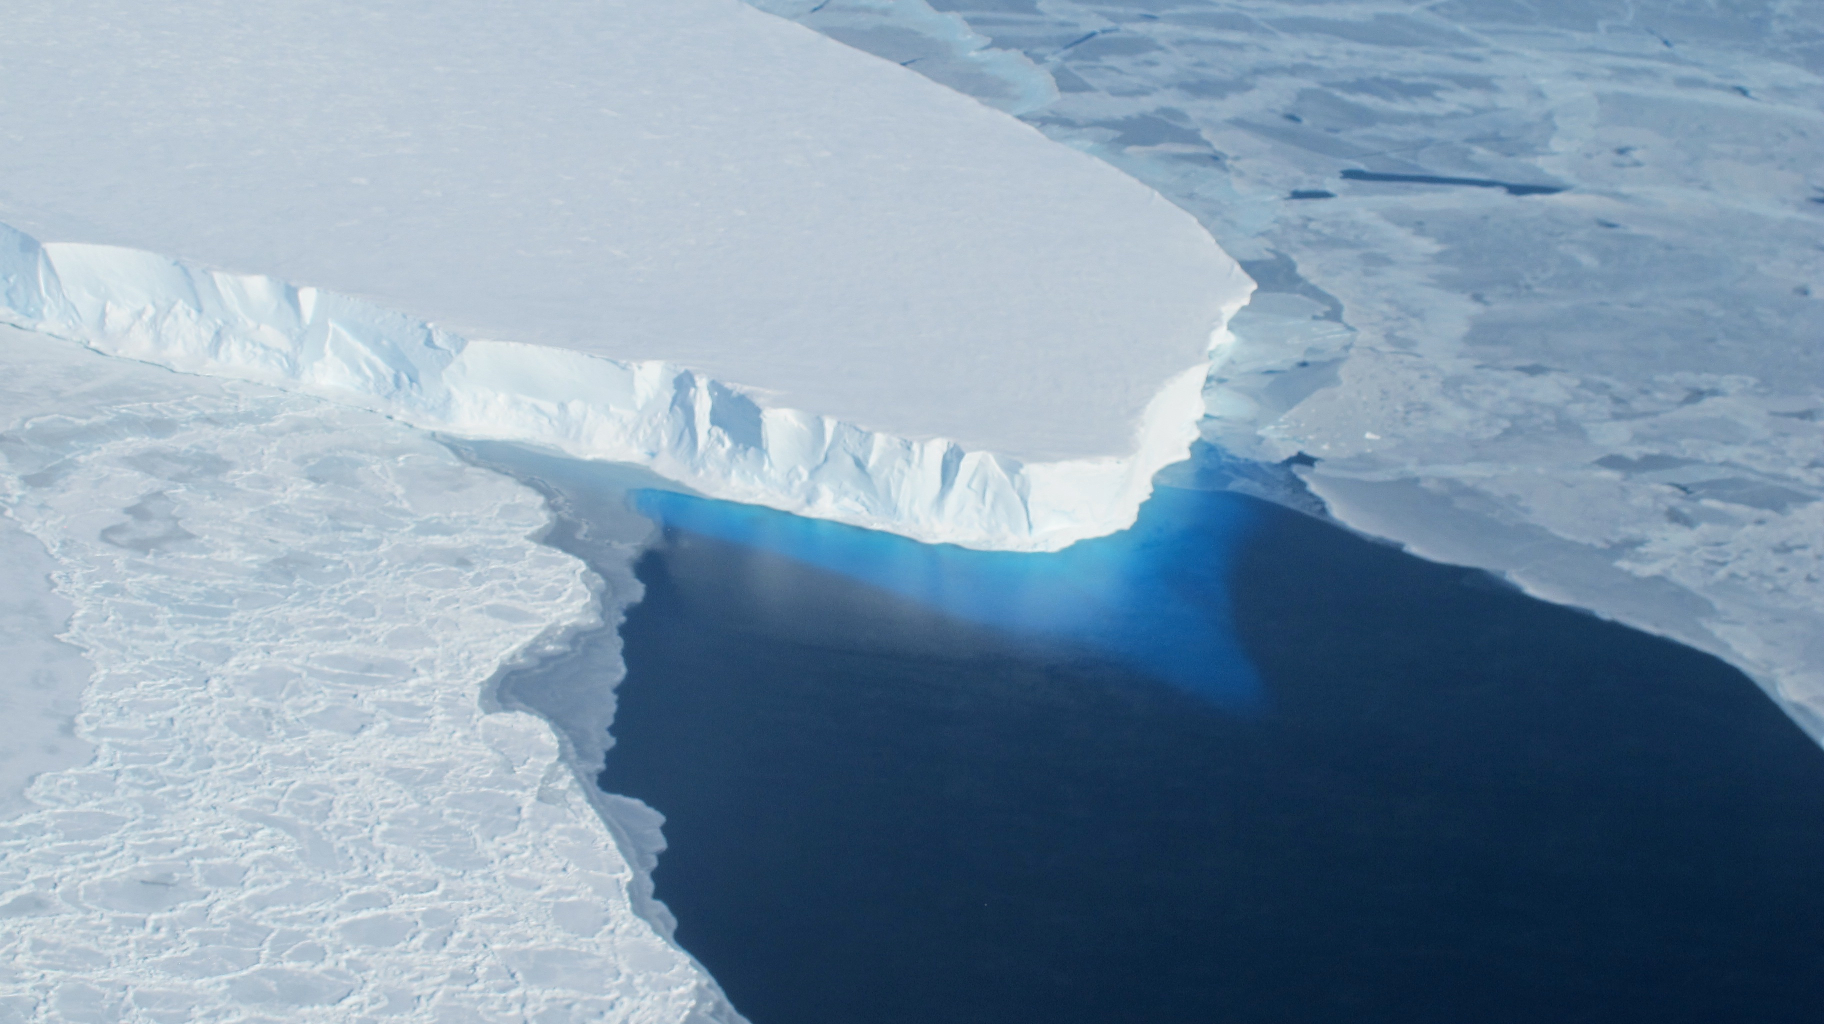
\includegraphics[width=1.0\textwidth]{supp4rignot-small}

\medskip
\tiny [ice shelf at Thwaites Glacier, Antarctic]
\end{center}
\end{frame}


\begin{frame}
  \frametitle{how to understand these viscous flows?}
  \framesubtitle{(big picture question 3)}

\begin{columns}
\begin{column}{0.6\textwidth}
\begin{itemize}
\item ice sheets are worth studying as fluids
\item they have four outstanding properties as viscous flow problems:
  \begin{enumerate}
  \item \alert{slow}
  \item \alert{shear-thinning}
  \item \alert{shallow}
  \item \alert{contact slip}
  \end{enumerate}
\item other fluids in same category:
  \begin{itemize}
  \item[$\circ$] salad dressing (\emph{look for ``xanthan gum'' as ingredient})
  \item[$\circ$] blood (\emph{except not shallow})
  \end{itemize}
\end{itemize}
\end{column}
\begin{column}{0.4\textwidth}

\hfill 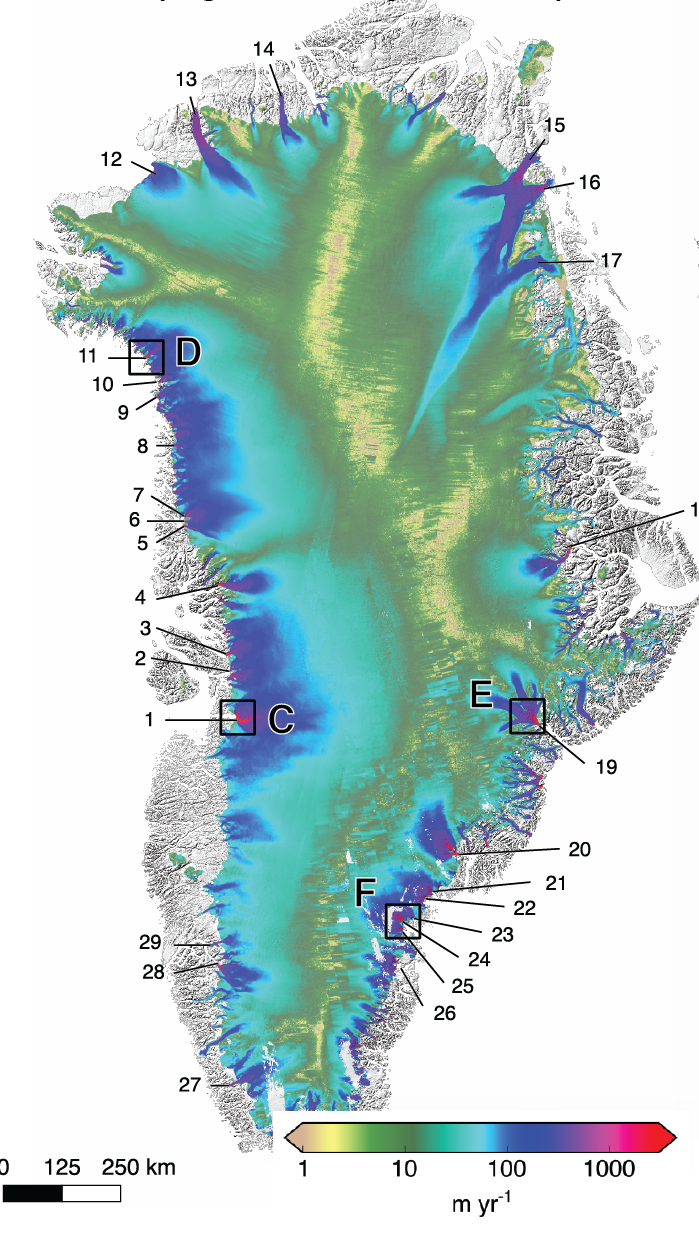
\includegraphics[width=0.95\textwidth]{greenland-overview-obsonly}
\end{column}
\end{columns}
\end{frame}


\section[numerical models]{numerical models of ice sheets}


\begin{frame}
  \frametitle{the major variables}

\begin{center}
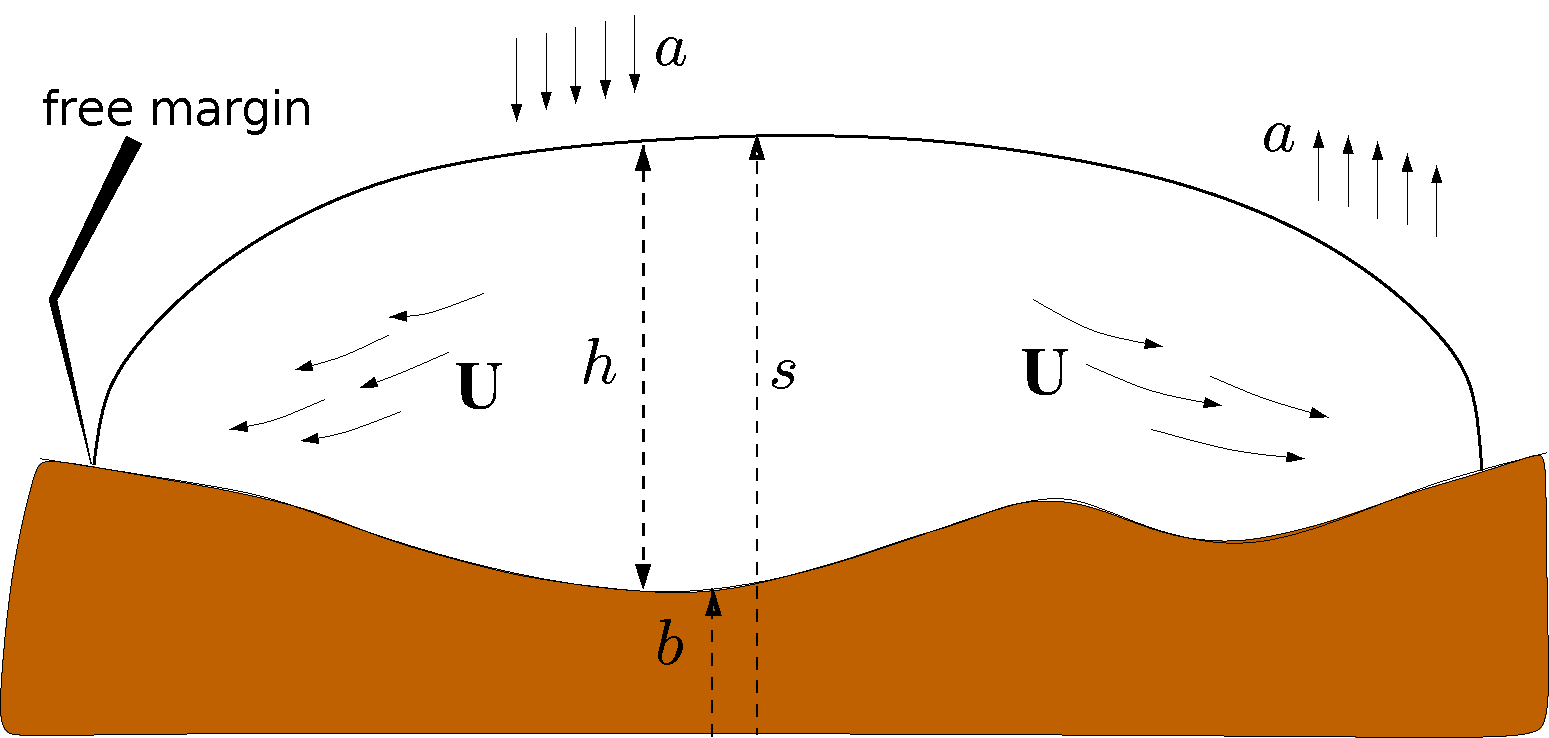
\includegraphics[width=0.7\textwidth]{groundedscheme}
\end{center}

\begin{itemize}
\small
\item $s=$ ice surface elevation
\item $b=$ bedrock elevation
\item $h=$ ice thickness $ = s-b$
\item ${\bf u}=$ velocity field
\item $a=$ surface mass balance (accumulation)

\bigskip
\item obvious(?) idea: ice surface $s$ is always above the bedrock $b$
\end{itemize}

\end{frame}


\begin{frame}
  \frametitle{shallow ice approximation (SIA)}

\begin{itemize}
\item recall standard Glen-Stokes model:
\small
\begin{align*}
\nabla \cdot \mathbf{u} &= 0 &&\text{\emph{incompressibility}} \\
0 &= - \nabla p + \nabla \cdot \tau_{ij} + \rho \mathbf{g} &&\text{\emph{stress balance}} \\
\mathbf{D}u_{ij} &= A \left|\tau_{ij}\right|^2 \tau_{ij} &&\text{\emph{Glen flow law}}
\end{align*}
\normalsize
\item \alert{most models don't solve it because it is too expensive}
\item derive SIA equations by scaling based on shallowness:
  \begin{itemize}
  \item[$\circ$] $[h]$ is a typical thickness, $[x]$ is a typical width
  \item[$\circ$] small parameter is $\eps = [h] / [x]$
  \end{itemize}
\item horizontal ice velocity is given by ($n=3$): 
  $${\bf U}  =  - \frac{2 A}{4} (\rho g)^{3} \left[ (s-b)^4 - (s - z)^4  \right] 
|\nabla s |^{2} \nabla s$$

\vspace{-2mm}
  \begin{itemize}
  \item[$\circ$] no PDE to solve for velocity
  \end{itemize}
\item SIA is good approximation when
  \begin{itemize}
  \item[$\circ$] sliding is small or zero
  \item[$\circ$] bedrock slope is modest
  \end{itemize}
\end{itemize}
\end{frame}



\begin{frame}
  \frametitle{steady state ice sheet geometry}

\begin{itemize}
\item mass conservation in steady state: 
  $$\Div \left(  \int_b^s {\bf U}\, dz \right)  =  a$$
\item shallow ice approximation + (steady) mass conservation:
\begin{equation}
- \Div \left(\Gamma (s-b)^5 | \nabla s |^2 \nabla s  \right) =  a  \tag{$\ast$}
\end{equation}
  \begin{itemize}
  \vspace{-0.2in}
  \item[$\circ$] this is the major SIA equation \dots a PDE
  \item[$\circ$] the unknown is ice surface elevation $s(x,y)$
  \item[$\circ$] like Poisson equation $-\Div (\nabla u) = f$ except nonlinear and singular
  \end{itemize}
\item the \alert{minimal useful numerical ice sheet model} is a program which approximately solves ($\ast$) for $s(x,y)$ given steady climate inputs $a(x,y)$ and bed elevation $b(x,y)$
\end{itemize}
\end{frame}


\begin{frame}
  \frametitle{obstacle problem: a mathematical analogy}

\begin{columns}
\begin{column}{0.35\textwidth}
\begin{itemize}
\item ice sheet surface \\ $\sim$ \alert{membrane}
\item bedrock $\sim$ \alert{obstacle}
\item ice sheet shape solves this kind of \alert{free boundary problem}
\end{itemize}
\vfill
\begin{center}
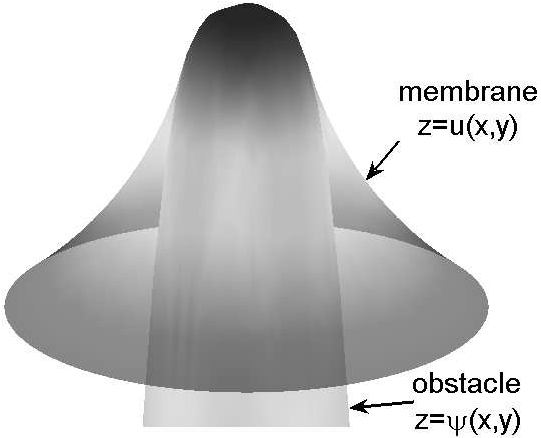
\includegraphics[width=1.0\textwidth]{classicalobs}
\end{center}
\end{column}
\begin{column}{0.65\textwidth}
\begin{center}
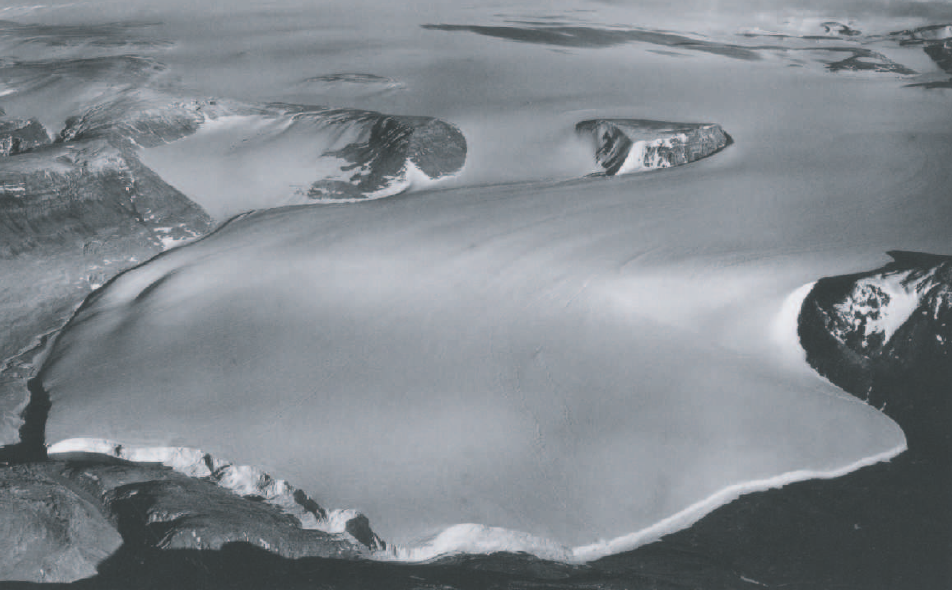
\includegraphics[width=0.8\textwidth]{polaris} \\
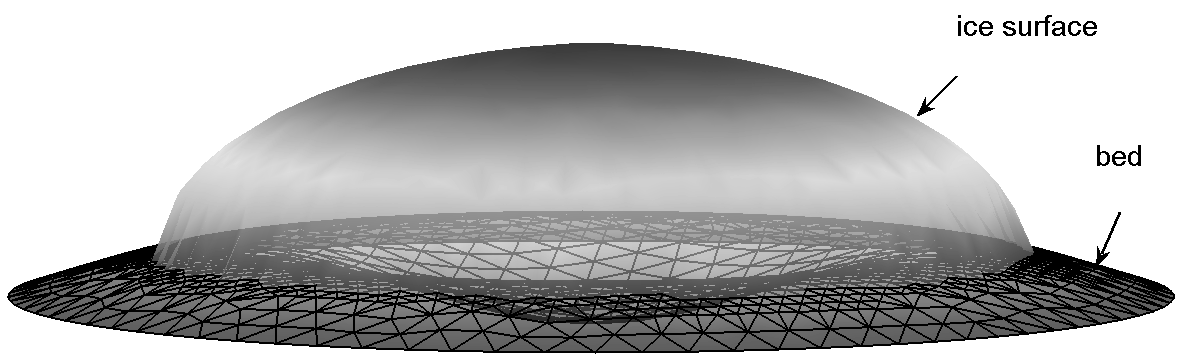
\includegraphics[width=\textwidth]{capnonflatobs}
\end{center}
\end{column}
\end{columns}
\end{frame}



\contactslipslide{recall this slide:}


\begin{frame}
  \frametitle{ice streams: another analogy}

\begin{columns}
\begin{column}{0.6\textwidth}
\begin{itemize}
\item ice streams emerge where basal resistance is low enough
\item basal resistance is low if there is pressurized liquid water at the ice base
\item the ice is a membrane which connects sliding parts to non-sliding parts

\bigskip
\item<2> note: ice \emph{shelves} have zero basal resistance
\item<2> the equations for ice streams and shelves are similar \dots more PDEs \dots which I'll skip
\end{itemize}
\end{column}
\begin{column}{0.4\textwidth}
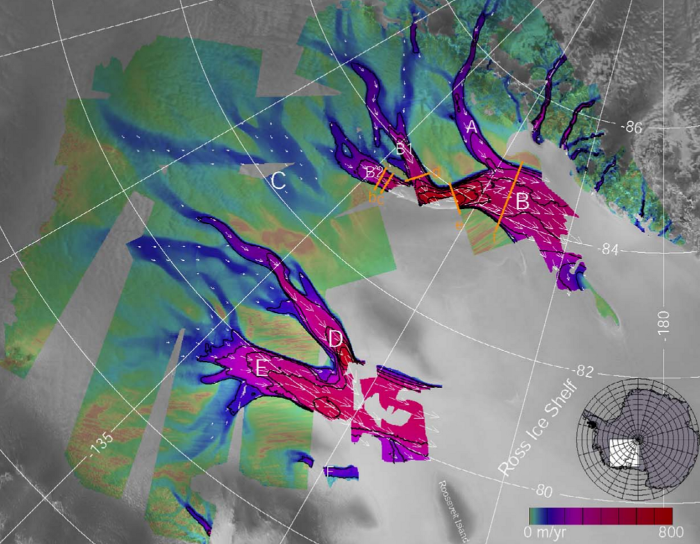
\includegraphics[width=\textwidth]{siple}

\vspace{0.3in}

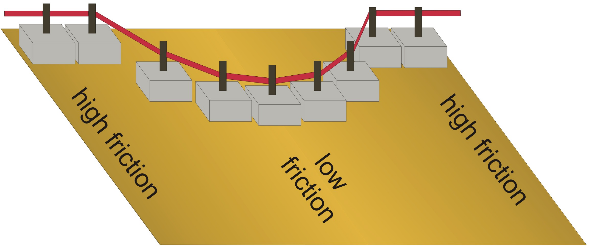
\includegraphics[width=1.1\textwidth]{schoof-sliders}
\end{column}
\end{columns}
\end{frame}


\begin{frame}{numerical model results: Greenland scenarios}

\begin{itemize}
\item for thinking about climate possibilities the IPCC proposed \emph{representative concentration pathways} for greenhouse gases in the next century
    \begin{itemize}
    \item[$\circ$] RCP 2.6 assumes least greenhouse gases
    \item[$\circ$] RCP 8.5 assumes most (``business as usual'')
    \item[$\circ$] consensus in 2014: mean sea level projected to rise by 0.26--0.82 m by 2100
    \item[$\circ$] even for 100 years, ice sheet behavior is the largest uncertainty
        \begin{itemize}
        \item uncertainty increases greatly thereafter
        \end{itemize}
    \end{itemize}
\item \alert{the following movie} is unpublished, new results
    \begin{itemize}
    \item[$\circ$] by Andy Aschwanden, a glaciologist here at UAF
    \item[$\circ$] using the Parallel Ice Sheet Model (PISM), developed here at UAF
        \begin{itemize}
        \item \url{www.pism-docs.org}
        \end{itemize}
    \item[$\circ$] shows next 1000 years for Greenland
    \end{itemize}
\end{itemize}
\end{frame}


\section[on being right]{how to know if numerical models are right?}

\begin{frame}{how to know if numerical models are right?}

\begin{itemize}
\item they are \emph{never} ``correct'' in the sense of ``exact match to reality'' \emph{or even} ``exact match to continuum equations''
\item the \alert{goal} is: \alert{close to exact, with knowable maximum errors, and rapidly converging with increasing computational effort}

\bigskip
\item<2> there are three basic strategies to be right:
    \begin{enumerate}
    \item proofs that a scheme converges or is stable (\emph{a priori} proofs)
    \item \alert{verification}: using known exact solutions of the equations to measure numerical error
    \item \alert{validation}: using well-measured real systems to measure numerical and model error
    \end{enumerate}
\end{itemize}
\end{frame}


\begin{frame}{need for exact solutions}

\begin{itemize}
\item verification is key tool to assist development of complex models
\item \alert{but requires exact solutions}
\item these come from:
    \begin{itemize}
    \item[$\circ$] exploiting symmetries and special configurations
        \begin{itemize}
        \item \alert{movie on nex slide} shows an example
        \end{itemize}
    \item[$\circ$] ``manufacturing'' solutions to differential equations by deriving inputs (source terms) using assumed formulas for solutions
    \end{itemize}
\item job security for applied mathematicians
\end{itemize}
\end{frame}


\begin{frame}{movie of time-dependent SIA}

\begin{itemize}
\item the Halfar similarity solution is an exact, time-dependent, zero mass balance solution where the $t\to 0^+$ limit is a delta function
\end{itemize}

\begin{center}
\includegraphics<1>[width=0.75\textwidth]{../../old/commonfigs/animhalfar/halfar0}

\includegraphics<2>[width=0.75\textwidth]{../../old/commonfigs/animhalfar/halfar1}

\includegraphics<3>[width=0.75\textwidth]{../../old/commonfigs/animhalfar/halfar2}

\includegraphics<4>[width=0.75\textwidth]{../../old/commonfigs/animhalfar/halfar3}

\includegraphics<5>[width=0.75\textwidth]{../../old/commonfigs/animhalfar/halfar4}

\includegraphics<6>[width=0.75\textwidth]{../../old/commonfigs/animhalfar/halfar5}

\includegraphics<7>[width=0.75\textwidth]{../../old/commonfigs/animhalfar/halfar6}

\includegraphics<8>[width=0.75\textwidth]{../../old/commonfigs/animhalfar/halfar7}

\includegraphics<9>[width=0.75\textwidth]{../../old/commonfigs/animhalfar/halfar8}

\includegraphics<10>[width=0.75\textwidth]{../../old/commonfigs/animhalfar/halfar9}

\includegraphics<11>[width=0.75\textwidth]{../../old/commonfigs/animhalfar/halfar10}

\includegraphics<12>[width=0.75\textwidth]{../../old/commonfigs/animhalfar/halfar11}

\includegraphics<13>[width=0.75\textwidth]{../../old/commonfigs/animhalfar/halfar12}

\includegraphics<14>[width=0.75\textwidth]{../../old/commonfigs/animhalfar/halfar13}
\end{center}

\vspace{-4mm}
\only<1>{\texttt{t=0.3 years}}
\only<2>{\texttt{t=1 year}}
\only<3>{\texttt{t=3 years}}
\only<4>{\texttt{t=10 years}}
\only<5>{\texttt{t=30 years}}
\only<6>{\texttt{t=100 years}}
\only<7>{\texttt{t=300 years}}
\only<8>{\texttt{t=1000 years}}
\only<9>{\texttt{t=3000 years}}
\only<10>{\texttt{t=10,000 years}}
\only<11>{\texttt{t=30,000 years}}
\only<12>{\texttt{t=100,000 years}}
\only<13>{\texttt{t=300,000 years}}
\only<14>{\texttt{t=1,000,000 years}}
\end{frame}


\begin{frame}{models of ice shelves: they work}

\begin{itemize}
\item Ross ice shelf (Antarctica) velocity below
  \begin{itemize}
  \item[$\circ$] observed versus computed by SSA model in PISM
  \item[$\circ$] tuned: single, constant $A$
  \end{itemize}
\end{itemize}
\vspace{-0.3in}

\begin{center}
  \mbox{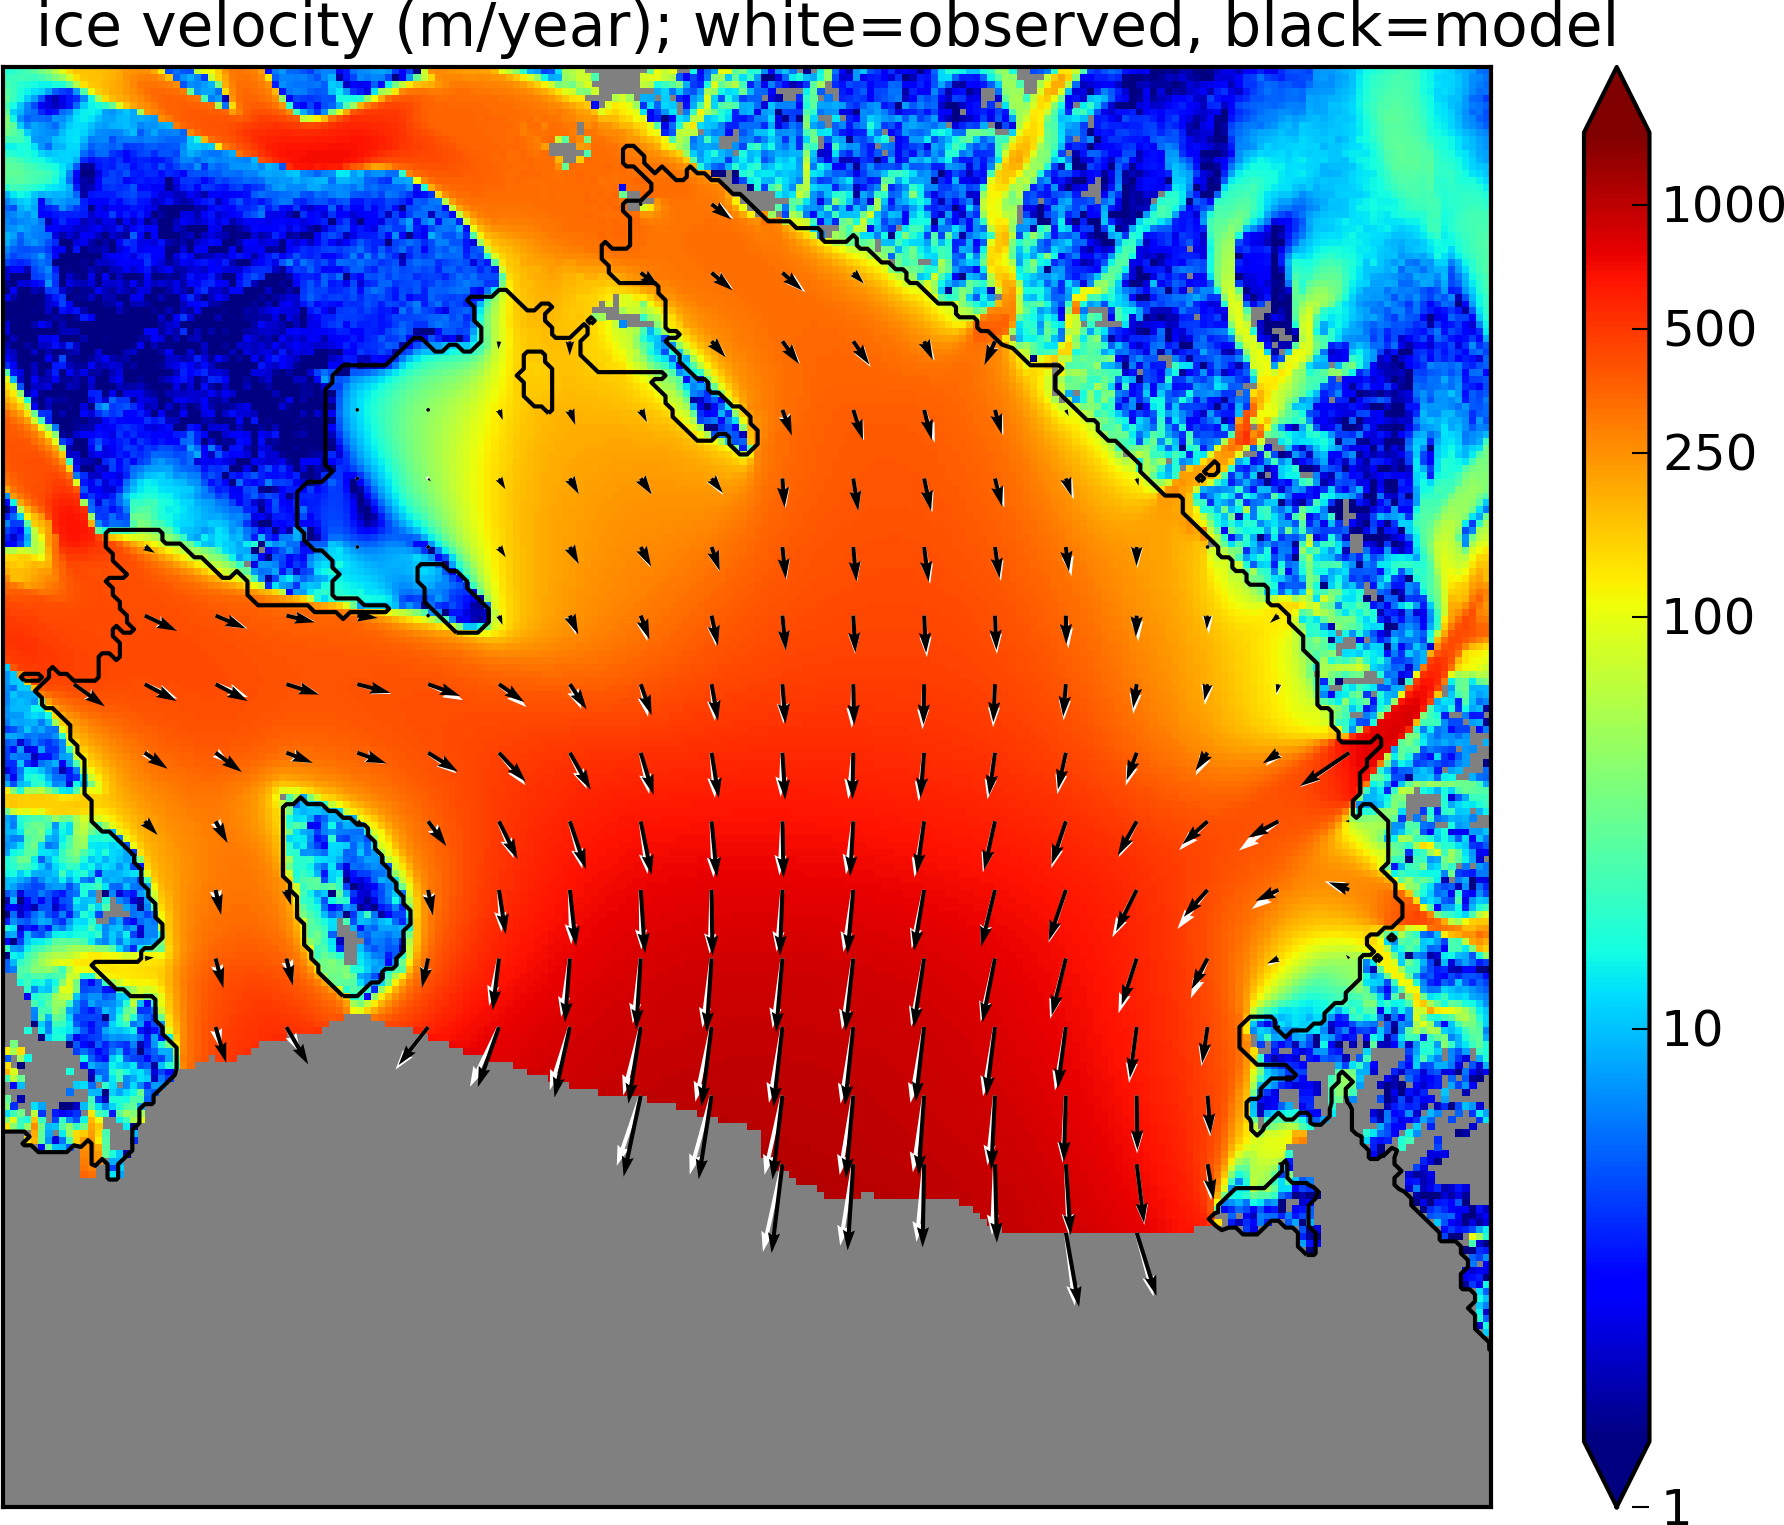
\includegraphics[width=0.58\textwidth]{rossquiver} \, 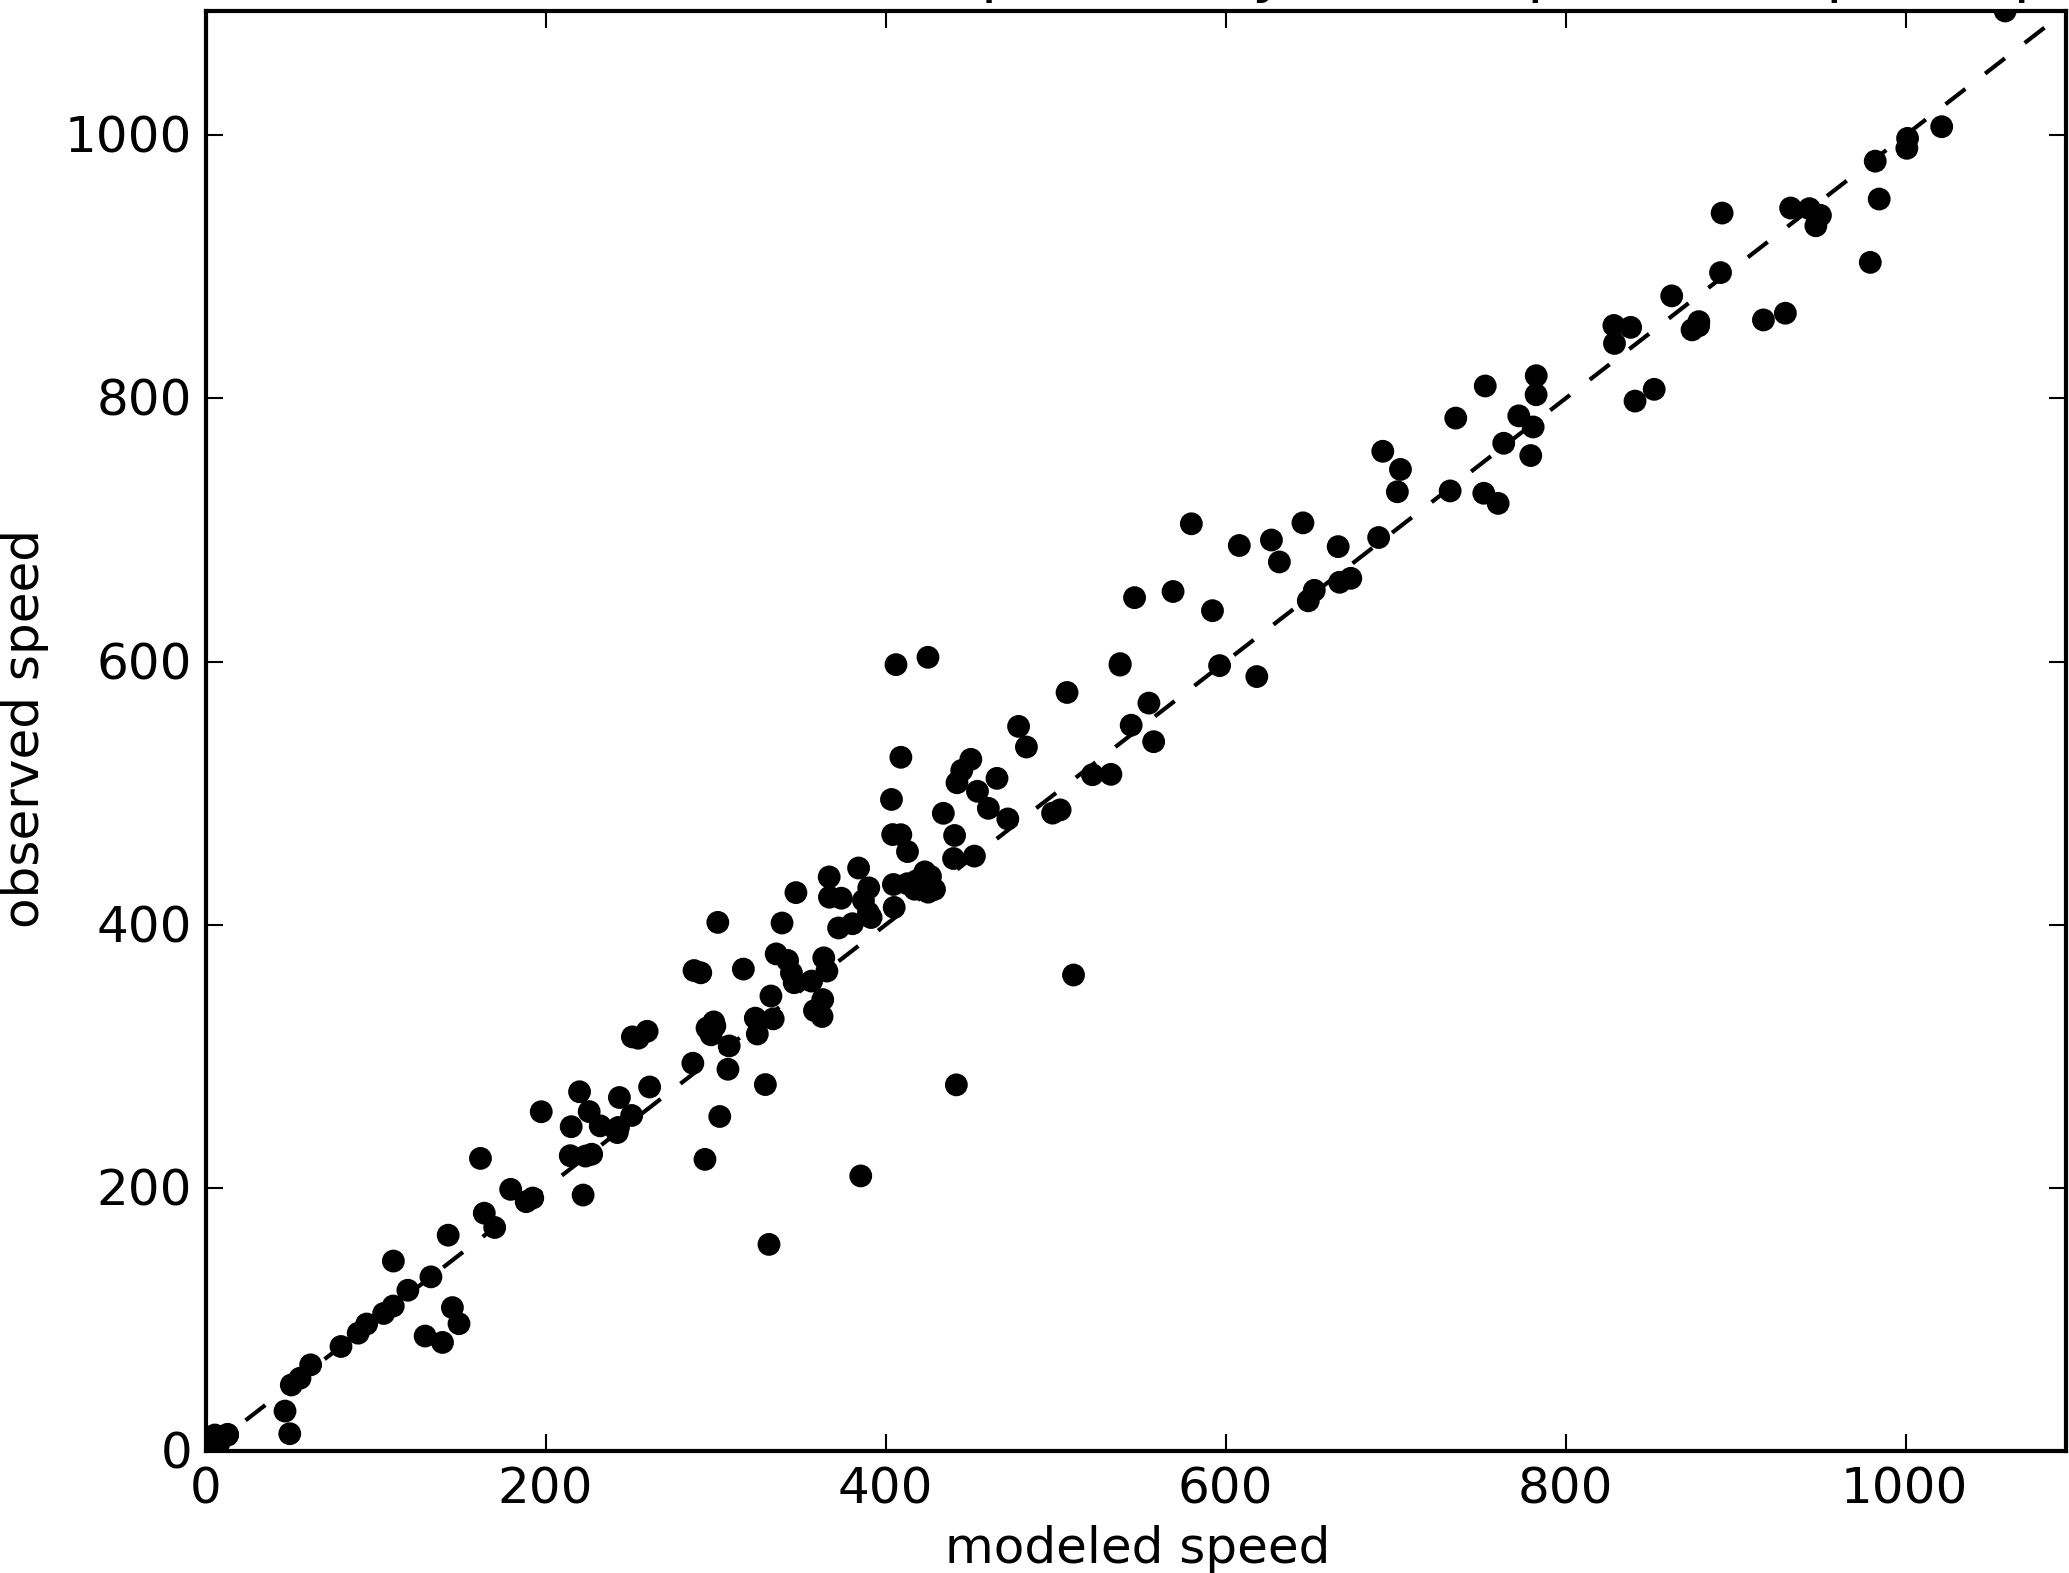
\includegraphics[width=0.48\textwidth]{rossscatter}}
\end{center}
\end{frame}

\begin{frame}
  \frametitle{moving grounding line in the lab}
  \framesubtitle{by Pegler et al.~(2014)}

\begin{center}

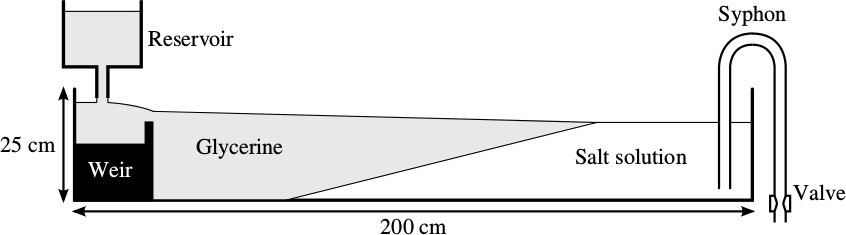
\includegraphics[width=0.7\textwidth]{pegler2014-grounding-line-schematic}

\vspace{1.0in}
[show movie]
\end{center}
\end{frame}


\section*{conclusion}

\begin{frame}
  \frametitle{conclusion}
  \framesubtitle{thanks for listening!}

\begin{itemize}
\item ice sheets are fluid problems
\item \dots for which the equations are systems of nonlinear PDEs
\item \dots so numerical models are needed in practice
\item \dots so it's a good field in which to work as an applied mathematician
\end{itemize}

\begin{center}
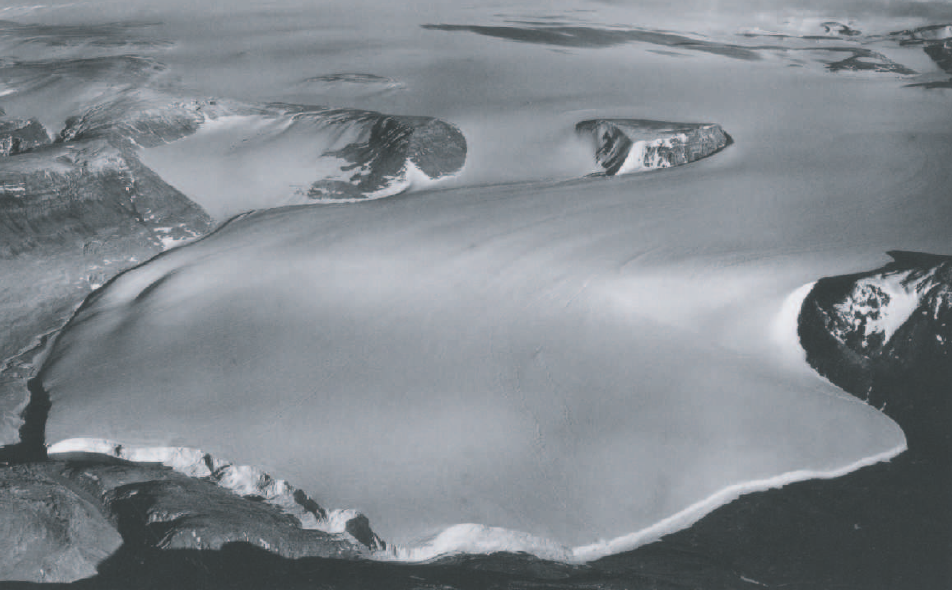
\includegraphics[width=0.6\textwidth]{polaris}
\end{center}
\end{frame}


\end{document}
